\chapter{Resultados Experimentales}


\section{Entorno de pruebas}
Para hacer las pruebas en la placa se ha utilizado la FPGA Artix-7 con placa Basys3, ya que se utiliza la misma en el estudio en el que se basa el proyecto\cite{desai2021low}.

El problema que se encontró con el uso de la placa es que la ROM no podría almacenar 650000 filas de valores de punto flotante por lo que se probo un dieciseisavo de las pruebas totales que equivale a 40625.

Por lo que, para hacer la prueba con todos los samples, se requiere utilizar una FPGA con más recursos como la Virtex-7 VC709 Evaluation Platform.

\begin{figure}[h]
	\centering
	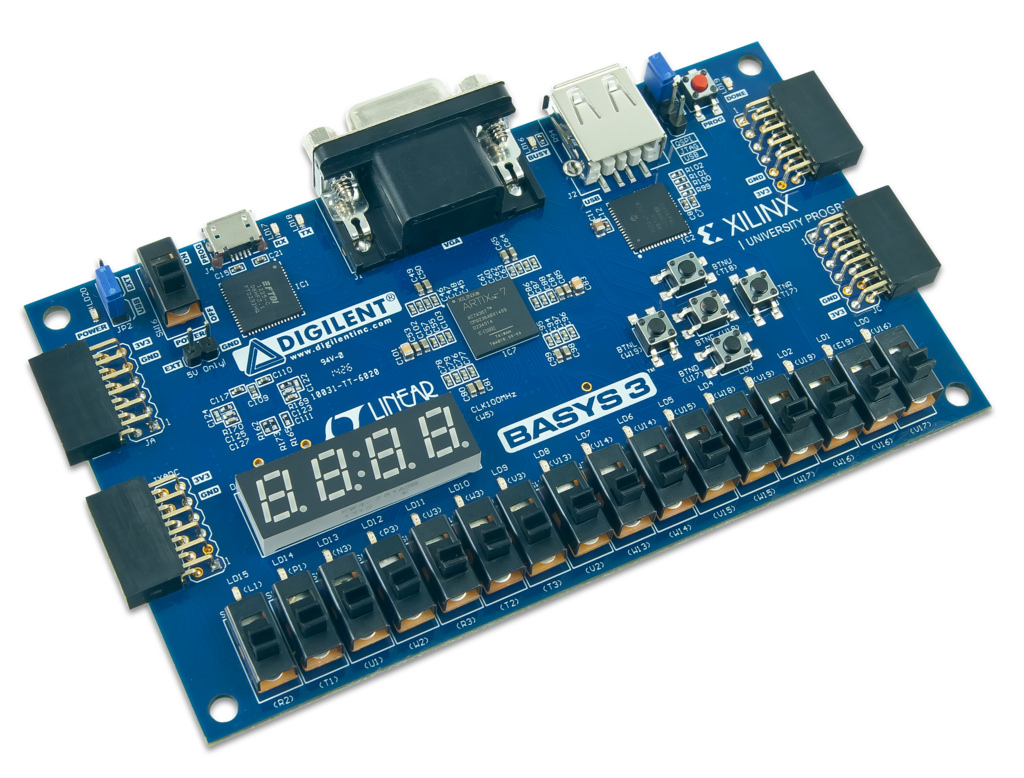
\includegraphics[width=0.6\textwidth]{./Images/img_introduccion/Basys3.jpg}
	\caption{Basys3 Artix-7 FPGA}
	\label{fig:Basys3}
\end{figure}

\section{Recursos necesarios}
	Para evaluar los recursos necesarios, se tendrán en cuenta los resultados sacados del análisis de síntesis, del reporte de  \textit{timing}  y del reporte de potencia del módulo principal que contiene el módulo de filtrado de señal,
	el módulo de detección de picos y el módulo de detección de arritmias. 
	
\subsection{Análisis de utilización}
En este reporte nos encontramos con los siguientes datos:

\begin{itemize}
    \item \textit{Slice LUTs}: Se utilizan 2016 de un total de 20800 disponibles. La mayoría de los LUTs se asignan a la parte de detección de picos, específicamente al módulo de división seguido del módulo de multiplicación en la parte del filtrado. El módulo de detección de arritmias apenas necesita LUTs en comparación con los otros módulos.
    \item \textit{Slice registers}: Se utilizan 3086 de un total de 41600 disponibles, y al igual que los LUTs, la mayoría se asignan a los módulos de división y multiplicación.
    \item Bloque \textit{RAM tile}: Se utiliza 1 tile de los 50 disponibles. La mitad se utiliza para la ROM de coeficientes y la otra mitad para la RAM de los valores de la señal original.
    \item Se utilizan 4 DSPs de los 90 disponibles. Dos de ellos se utilizan en el módulo de multiplicación y dos en el módulo restador.
\end{itemize}


\begin{figure}[h]
	\centering
	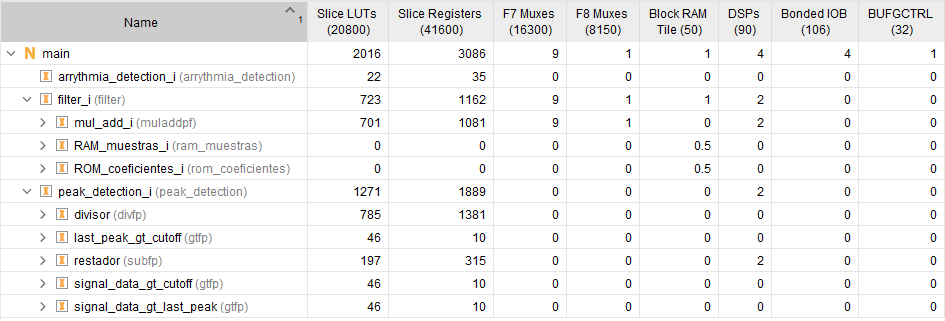
\includegraphics[width=0.99\textwidth]{./Images/img_res_experimentales/utilization1.png}
	\caption{Reporte total de utilización}
	\label{fig:utilization1}
\end{figure}

Se han utilizado menos de un 10\% del  \textit{hardware}  disponible para cada recurso.
\begin{figure}[h]
	\centering
	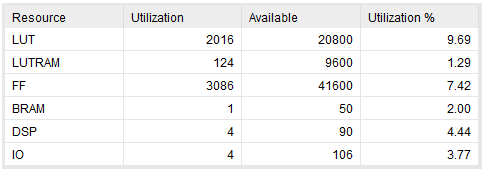
\includegraphics[width=0.6\textwidth]{./Images/img_res_experimentales/utilization2.png}
	\caption{Porcentaje del reporte total de utilización}
	\label{fig:utilization2}
\end{figure}

\begin{figure}[h]
	\centering
	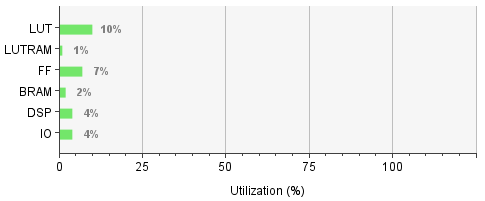
\includegraphics[width=0.6\textwidth]{./Images/img_res_experimentales/utilization3.png}
	\caption{Reporte total de utilización}
	\label{fig:utilization3}
\end{figure}


\subsection{Análisis de \textit{timing} }

La frecuencia de funcionamiento se ha calculado según la referencia del artículo \cite{desai2021low}, que indica que las muestras se toman a 360 sps (\textit{samples per second}), lo que equivale a 360 Hz. Con esta información, sabemos que una muestra llega cada \( \frac{1}{360 Hz} = 2.777 ms\).

También se calcula el número de ciclos que tarda en ejecutarse el módulo de filtrado, que resulta ser el más crítico de todos. Este módulo requiere un total de 1780 ciclos, por lo que \( \frac{2.777  ms}{1780 ciclos} = 1.56  microsegundos \) por ciclo. Por lo tanto, en el \textit{waveform} se establecerá un periodo de 1500 ns con una oscilación desde 0 a 750 ns para que sea simétrico.


\lstset{language=VHDL, breaklines=true, basicstyle=\footnotesize}
\begin{lstlisting}[frame=single]
## Clock signal
set_property PACKAGE_PIN W5 [get_ports clk]							
	set_property IOSTANDARD LVCMOS33 [get_ports clk]
	create_clock -add -name sys_clk_pin -period 1500.00 -waveform {0 750} [get_ports clk]
\end{lstlisting}

	En el análisis de  \textit{timing}  se comprobará cuál es el \textit{worst negative slack} y se calculará el periodo mínimo necesario. Este reporte de  \textit{timing}  muestra lo siguiente. La frecuencia alcanzada con ese periodo es de 0,540 MHz

	\begin{figure}[h!]
		\centering
		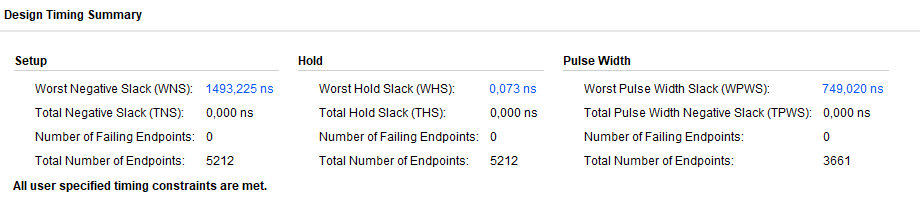
\includegraphics[width=0.9\textwidth]{./Images/img_res_experimentales/reportetiming.png}
		\caption{Imagen que muestra el reporte de  \textit{timing}  generado}
		\label{fig:reporteTiming}
	\end{figure} 

	Para calcular el periodo mínimo necesario se resta el periodo actual menos el \textit{worst negative slack} dando como resultado 6,775 ns de periodo mínimo de funcionamiento.  
	\[f - wns = f{min}\]
	\[1500 - 1493,225 = 6,775\]

	

\subsection{Análisis de potencia}

	En el análisis de potencia se evalúa la potencia que necesita la FPGA para poder llevar a cabo la ejecución.

	\begin{figure}[h!]
		\centering
		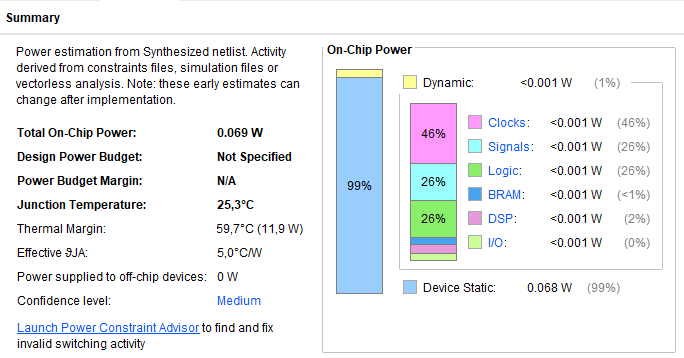
\includegraphics[width=0.6\textwidth]{./Images/img_res_experimentales/reportepower.png}
		\caption{Imagen que muestra el reporte de potencia generado}
		\label{fig:reportepotencia}
	\end{figure} 

	En este análisis la potencia alcanzada es de 0,069 W, pero casi todo el consumo es causado por la placa en sí (Device static), este algoritmo no gasta más de un 0,001 Vatios como se puede ver en la \cref*{fig:hierarchical} del \textit{hardware} utilizado a temperatura ambiente como se ve en la \cref*{fig:temperaturaambiente}

	\begin{figure}[h!]
		\centering
		\includegraphics[width=0.6\textwidth]{./Images/img_res_experimentales/temperaturaambientereportepower.png}
		\caption{Imagen que muestra la temperatura con la que desempeña el consumo generado}
		\label{fig:temperaturaambiente}
	\end{figure} 

	\begin{figure}[h!]
		\centering
		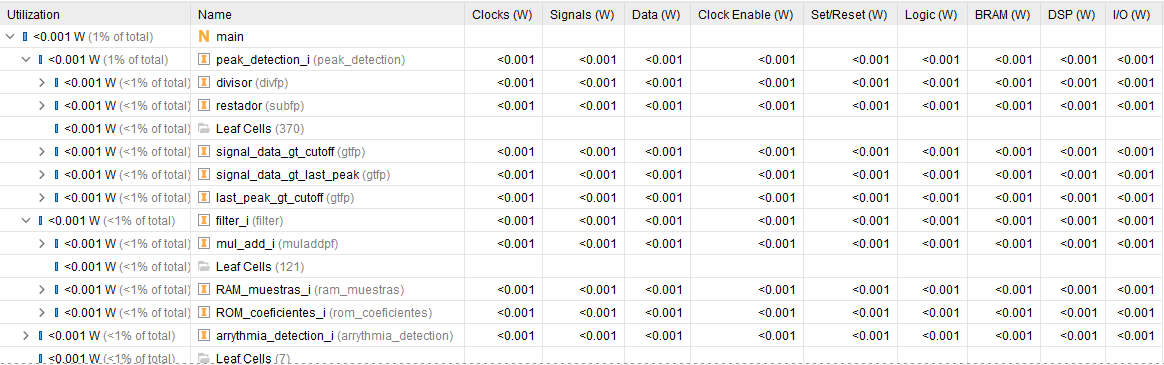
\includegraphics[width=0.99\textwidth]{./Images/img_res_experimentales/hierarchical.png}
		\caption{Muestra el total consumo de todos los componentes generados en  \textit{hardware} }
		\label{fig:hierarchical}
	\end{figure} 

	\begin{figure}[h!]
		\centering
		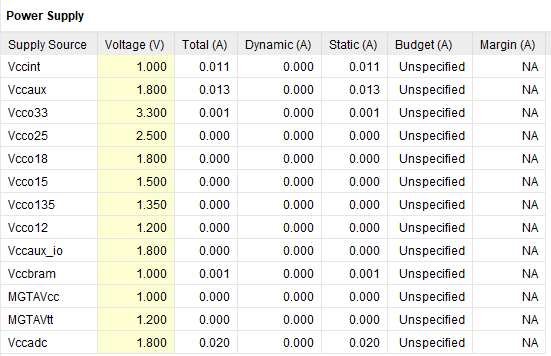
\includegraphics[width=0.9\textwidth]{./Images/img_res_experimentales/powersupply.png}
		\caption{Muestra el power supply}
		\label{fig:powersupply}
	\end{figure} 
	\FloatBarrier

	Analizando más a fondo el consumo, se puede comprobar que el \textit{signal rate} de la lógica no traspasa los 0,5 Mtr/s, el de la BRAM y los DSP también son bajos.
	
	\begin{figure}[h!]
		\centering
		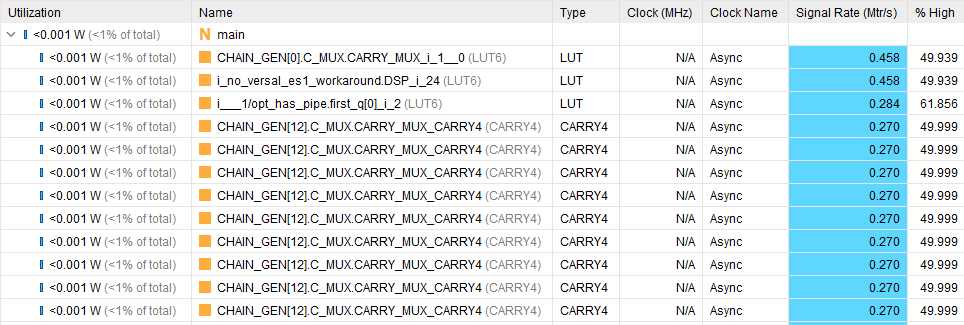
\includegraphics[width=0.6\textwidth]{./Images/img_res_experimentales/signalratelogic.png}
		\caption{Imagen que muestra la el signal rate de la lógica}
		\label{fig:signalratelogic}
	\end{figure} 

	\begin{figure}[h!]
		\centering
		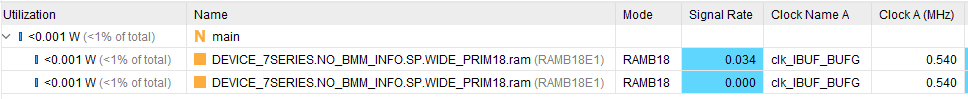
\includegraphics[width=0.6\textwidth]{./Images/img_res_experimentales/signalrateBRAM.png}
		\caption{Imagen que muestra la el signal rate de BRAM}
		\label{fig:signalrateBRAM}
	\end{figure} 

	\begin{figure}[h!]
		\centering
		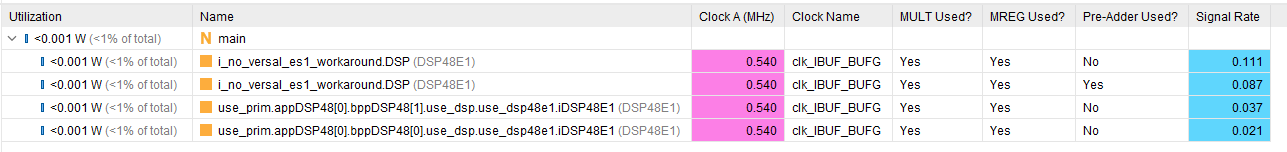
\includegraphics[width=0.6\textwidth]{./Images/img_res_experimentales/signalrateDSP.png}
		\caption{Imagen que muestra la el signal rate de los DSP}
		\label{fig:signalrateDSP}
	\end{figure} 

	Comparando este proyecto con otros estudios, por ejemplo con el de caracterización de señales usando polinomios de Hermite \cite{desai2021low} presentan unos resultados de potencia de 28mW. Lo que hace nuestro algoritmo significativamente mejor en términos de consumo.








	